\cleardoublepage
\chapter{DEMONSTRASI GUARD RAIL PROTOTIPE}
\label{lamp:prototipe-guardrail}

Lampiran ini melengkapi pembahasan prototipe pada Bab~\ref{chap:implementasi}, khususnya mekanisme \textit{guard rail} keyakinan yang dijelaskan pada Subbab~\ref{subsec:impl-guardrail}. Tujuannya adalah memperlihatkan perilaku sistem ketika menerima pertanyaan yang berada di luar cakupan korpus PubMedQA.

Gambar~\ref{fig:lowconfidence} menampilkan tangkapan layar prototipe ketika diberi pertanyaan umum yang tidak berkaitan dengan bukti ilmiah pada korpus, yaitu \textit{``is it okay to take medicine without eat first?''}. Untuk pertanyaan tersebut, dokumen yang ditarik oleh tahap \textit{retrieval} memiliki skor relevansi yang rendah, sehingga skor keyakinan komposit hanya bernilai 16\% dan masuk ke kategori rendah.

\begin{figure}[H]
  \centering
  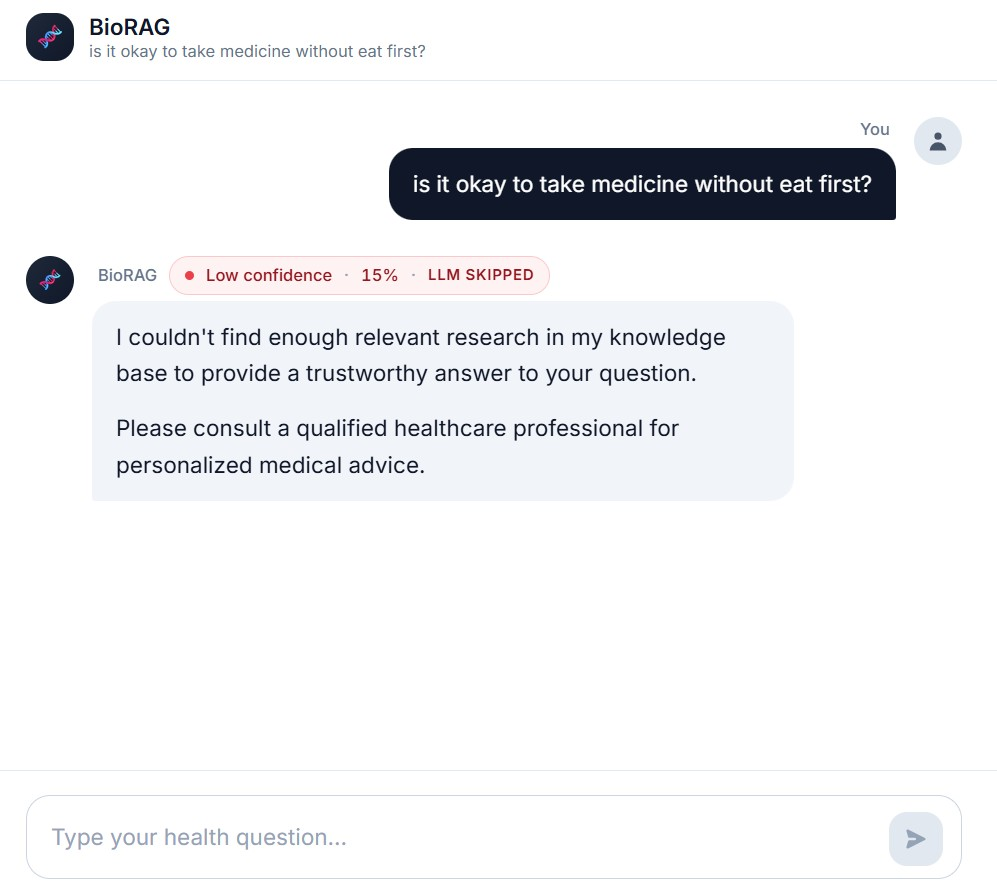
\includegraphics[width=0.9\textwidth]{image/lowconfidencescore.jpg}
  \caption{Perilaku \textit{guard rail} pada pertanyaan di luar cakupan korpus: skor keyakinan rendah (16\%) sehingga pemanggilan LLM dilewati}
  \label{fig:lowconfidence}
\end{figure}

Karena skor berada pada kategori rendah, sistem tidak meneruskan pertanyaan ke LLM, melainkan menampilkan penanda \textit{Low confidence} beserta keterangan \textit{LLM SKIPPED}, lalu mengembalikan pesan bahwa sistem tidak menemukan bukti yang cukup untuk memberikan jawaban tepercaya dan menyarankan pengguna berkonsultasi dengan tenaga medis. Perilaku ini menunjukkan bahwa \textit{guard rail} berfungsi sebagai lapisan pengaman tambahan, yaitu menahan sistem dari memberikan jawaban yang berpotensi mengandung halusinasi ketika konteks pendukung tidak memadai.
